\section{Übersicht}
\setauthor{Stefano Pyringer}

Diese Abbildung bietet einen groben Überblick über die Technologien, die für die Erstellung und Betrieb der Feedback App verwendet wurden.
Für die Umsetzung der Applikation wurde die Programmiersprache C\# verwendet. Die Technologien werden in Kapitel 3 ausführlich erklärt.

\begin{figure} [h]
    \begin{center}
        \includegraphics*[width=15cm]{./pics/architecture_overview.png}
        \caption[overview architecture]{Systemarchitektur Überblick \cite{CSharpLogo} \cite{XamarinLogo}}
    \end{center}
\end{figure}

\subsubsection{Backend}
\begin{itemize}
    \item .NET 6
    \item \begin{itemize}
        \item ASP.NET Core
        \item Entity Framework Core
        \item ASP.NET Core Identity
    \end{itemize}
\end{itemize}

Für das Backend wurde die Software-Entwicklungsplattform .NET 6 verwendet, um Datenstruktur, Repositories und Authentifizierung zu realisieren. 
Es wird mittels HTTP-API mit dem Frontend kommuniziert.

\subsubsection{Frontend}
Das Frontend handhabt die Interaktionen des Benutzers und stellt die von der API zur Verfügung gestellten Daten dar. Der Client ist auf mobilen Endgeräten 
mit dem Betriebssystem Android und iOS lauffähig. Das Frontend wurde mit Xamarin realisiert.

\section{Backend}
\setauthor{Stefano Pyringer}
\subsection{Datenstruktur}
\setauthor{Stefano Pyringer}

\begin{figure}[h]
    \begin{center}
        \includegraphics*[width=12cm]{./pics/FeedbackDb-ERD.png}
    \caption[ERD FeedbackDb]{FeedbackDb Entity Relationship Diagramm}
    \end{center} 
\end{figure}

\subsubsection{Tabelle Feedback}
Diese Tabelle beschreibt das Feedback für eine Lehreinheit. Der User kann die Lehreinheit in Sternen (1-5) bewerten und einen Kommentar hinzufügen. 

\subsubsection{Tabelle User}
Beinhaltet alle zusätzlichen personenbezogene Daten des Benutzers und die Rolle. Der Fremdschlüssel IdentityId verbindet die Tabelle 1:1 zu der User-Tabelle 
der Identity-Datenbank. Der User kann mehrere Feedbacks und Lehreinheiten erstellen. Je Benutzer ist eine Statistiktabelle verbunden.

\subsubsection{Tabelle TeachingUnit}
Es ist die Hauptkomponente der gesamten Datenbank. Hier werden alle notwendigen Daten gespeichert, die für das Erstellen einer Lehreinheit notwendig sind. 
Sie ist verbunden mit mehreren Feedbacks von anderen Usern und ist mit einer Tabelle für die Statistiken der Lehreinheit verbunden.

\subsubsection{Tabelle TeachingUnitStats}
Die Statistik für eine Lehreinheit speichert die Anzahl der gegebenen Feedbacks und die durchschnittliche Bewertungszahl einer Lehreinheit.

\subsubsection{Tabelle UserStats}
Diese Tabelle beinhaltet Statistiken für einen User. Es werden die Anzahl der erstellten Lehreinheiten und Bewertungen mit deren durchschnittlichen Bewertungszahl erfasst.

\subsubsection{Tabelle GlobalHistory}
Die globale Statistik Tabelle zählt alle jemals erstellten Lehreinheiten und Bewertungen des Servers an. Diese sind öffentlich zugänglich. 
D. h. es ist keine Autorisierung  notwendig.

\subsubsection{ASP.NET CORE Identity}
Die Daten für die ASP.NET Core Identity Authentifizierungsschnittstelle ist in der SarathalDb realisiert. Die Tabellen 
entsprechen dem vorgefertigten Schemas des NuGet-Package.

\begin{figure}[h]
    \begin{center}
        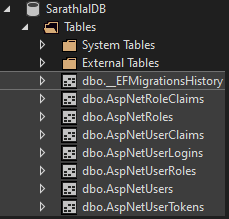
\includegraphics[width=8cm]{./pics/identity_tables.png}
        \caption[Identity Tables]{Tabellen der Idendity Datenbank}
    \end{center}
\end{figure}

\newpage
\subsection{Models}
\setauthor{Stefano Pyringer}
\begin{figure}[h]
    \begin{center}
        \includegraphics*[width=15cm]{./pics/models_FeedbackWebAPI.png}
        \caption[models API]{Model Feedback Web-API | links oben: Feedback, links unten: AccountManagement, rechts: Feedback}
    \end{center}
\end{figure}

Diese Models dienen als Schnittstelle für den Zugriff aus der HTTP-API zum Controller. Die Models definieren, welche Felder im HTTP-Body
einer HTTP-Request haben soll, um von der Methode angenommen zu werden. Zudem wird eine gewisse Sicherheit gewährleistet, da nur die definierten Felder 
erstellt oder bearbeitet werden dürfen.

\subsection{API-Services}
\setauthor{Stefano Pyringer}
Das Backend stellt einen API-Service für das Frontend zur Verfügung. Mittel HTTP-Requests können Daten empfangen und gesendet werden. 
Die Autorisierung  wird mittels Anhang eines JWT-Tokens realisiert. Die API-Methoden werden mit OpenAPI Swagger beschrieben und vereinfachte so die Entwicklung 
der HTTP-Zugriffsmethoden für das Frontend. Eine genaue Beschreibung der Umsetzung ist in Kapitel 6.1 zu finden.

\newpage
\section{Frontend}
\setauthor{Mirzet Sankonjic}

\subsection{Models}
Jedes Model ist ein Interface. In diesem Interface wird ein neues Datenmodel definiert,
welches in allen Componenten und Services verwendet werden kann. Dieses Datenmodel
ist ident mit den Data Transfer Objects oder Entitäten des Servers und dient als
Schnittstelle.
\subsection{Services}
Die Daten werden vom Client über einen Service per API an den Server gesendet
und wieder empfangen. Hierfür wird das HttpClientModule eingebunden. Es stehen
die HTTP-Requests GET, POST, PUT, PATCH und DELETE zur Verfügung. Die
Services werden dann in den benötigten Componenten injiziert im Konstruktor. Durch
die typisierte Variante wird ein Observable <> zurückgegeben.